% !TEX root =../main.tex
\chapter{Posicionamiento mediante marcadores visuales}\label{chp-01}


%%% Figuras %%%%
\def\figFlow{
%TODO: añadir conexión con autopiloto y pequeña descripción interna
%TODO: añadir imagen de cámara en su bloque 
\begin{figure}
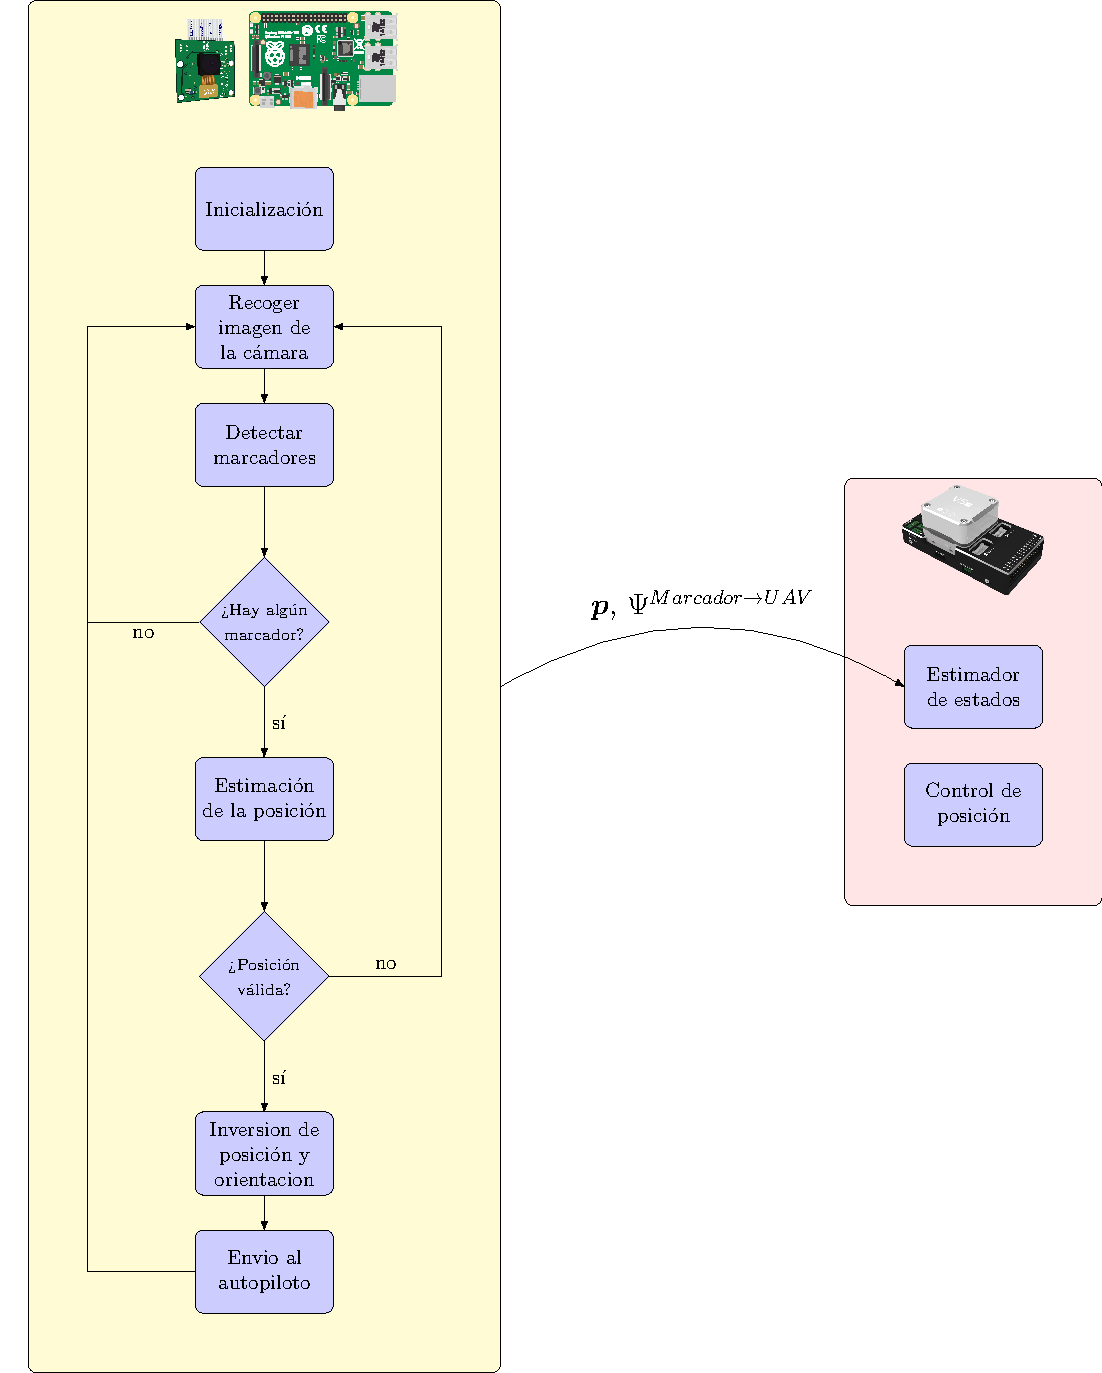
\includegraphics[width=\textwidth]{posicionamiento_marcadores/tikz/diagrama_flujo}
\caption{A la izquierda: diagrama de flujo del programa que se corre en el ordenador embebido, a la derecha: algunas de las tareas del autopiloto}
\label{fig:flow}
\end{figure}
}

\def\figEjes{
\begin{figure}
\includegraphics[width=\textwidth]{posicionamiento_marcadores/ejes}
\caption{Sistemas de referencia presentes en el problema}
\label{fig:ejes}
\end{figure}
}


% Más concretamente la precisión que se busca es centimétrica, pensando en coger un objeto metálico de manera autónoma con un imán colgando del UAV
\lettrine[lraise=-0.1, lines=2, loversize=0.2]{C}{onseguir} con precisión la posición de un vehículo aéreo no tripulado es bastante deseable. En la introducción se comentó aplicaciones como la manipulación de objetos o la navegación cerca de obstáculos. En este cápitulo se explica que para conseguirlo se ha construido un quadrotor con los componentes necesarios para detectar un marcador visual y cómo se ha programado un ordenador embebido en el quadrotor para que procese dicho marcador. 

De manera resumida, el funcionamiento es el siguiente:
- Se ha colocado un una cámara en la parte inferior del quadrotor, conectada a un ordenador embebido que procesa las imágenes tomadas
- En el suelo se coloca un marcador impreso que es detectado por la cámara
- Este le envía al autopiloto la posición y orientación del UAV con respecto a los ejes de coordenadas del del marcador 
- El autopiloto lo recibe, lo fusiona en su estimador de estados
- El estimador genera una posición estimada que alimenta al controlador de posición
- El controlador de posición toma esta medida y sigue la referencia. Esta última puede venir o bien del mando (consignas de movimiento en ejes inerciales) o del ordenador embebido el cual le indique una trayectoria.

Nótese que el controlador de posición también se podría haber ubicado en el ordenador embebido, generando consignas de aceleración en ejes cuerpo en función de los errores de posición en ejes cuerpo. La desventaja de esto es que se no se utilizan los demás sensores para el posicionamiento, por ejemplo si en un instante falta la medida de la visión, el autopiloto podría tomar otras como el acelerómetro, el GPS, el flujo óptico... 

\section{Mi programa}

\figFlow

%\begin{figure}
%\includegraphics[width=\textwidth]{posicionamiento_marcadores/pasosAruco}
%\caption{Pasos del proceso de detección de marcadores}
%\label{fig:pasosAruco}
%\end{figure}

- Inicialización: 
- Recoger imagen de la cámara: Este podría llegar a ser muy lento si no se escoge una interfaz con la cámara adecuada, por ejemplo USB. En este caso se ha escogido CSI que lleva la imagen directamente a la GPU y esta la lleva mediante DMA a la RAM. Todo ello sin consumir tiempo de CPU permitiendo que esta haga en paralelo otras operaciones como el procesamiento de imagen.
- Detectar marcadores: El objetivo es ubicar los marcadores de la imagen y extraer su identificador. Este proceso está explicado en \cite{aruco2014}, pero lo que se va a aportar aquí es una referencia directa al código de la librería aruco y a algunas funciones implementadas. 
	- 1. El primer paso es la extración de bordes a partir de la imagen convertida a blanco y negro. 
	- 2. A partir de la imagen binaria del paso anterior, se extraen los contornos usando en \textit{\_findMarkerContours()} la función de OpenCV  \textit{}
	- 3. Se realiza una aproximación poligonal y se quedan aquellos que solo estén compuestos por 4 puntos. 
- Estimación de la posición
	La estimación de la posición y la orientación se realiza tomando las esquinas de un marcador obtenido en el paso anterior.  
- Inversión de posición y orientación 
	Como se ve en la figura \ref{fig:ejes} hay varios sistemas de referencia que entran en juego y hay que tenerlos presente para tranformar desde lo que aporta la detección de marcadores hasta lo que necesita el autopiloto. En el paso anterior, la orientación y posición que se obtiene es la del \textbf{marcador con respecto a la cámara}, es decir se obtiene $R^{Marcador\rightarrow C\acute{a}mara}$ y $p^{Marcador\rightarrow C\acute{a}mara}$. En el código \ref{cod:inver} se puede ver que una vez obtenida dicha matriz de rotación esta se invierte o trasnpone para conseguir la orientación de la cámara vista desde el sistema de referencia del marcador. Dicha matriz se utiliza para expresar la posición del marcador en unos ejes rotados centrados en la cámara y paralelos a los ejes del marcador. Esta posición simplemente se niega para obtener la posición de la cámara vista desde el marcador $p^{C\acute{a}mara\rightarrow Marcador}$ que es la que se le envía al autopiloto. En cuanto a la orientación, como se ve en la figura, los ejes de la cámara y los del UAV están rotados 180\textdegree con respecto al eje z. Conociendo esto se obtiene la orientación del UAV visto desde el marcador:

	\begin{equation}
	R^{Marcador\rightarrow UAV}=\left( R^{C\acute{a}mara\rightarrow Marcador}\ R^{UAV\rightarrow C\acute{a}mara} \right)^T
	\end{equation}

	\figEjes

	\begin{codigo}{Inversión de la posición y orientación ubicada en mi archivo \textit{marker\_vison.h}}
	\label{cod:inver}
	\inputminted{c++}{posicionamiento_marcadores/cod_inver.cpp}[numberfirstline=281]
	\end{codigo} 

	% TODO: explicar rotación en ángulos de euler
	
- Envio al autopiloto 
	La orientación y la posición son enviadas a autopiloto a través del protocolo \textit{Mavlink}
	Una vez que las recive, este calcula la rotación entre su orientación expresada en ejes NED y su orientación expresada en el sistema de referencia de la visión, que en este caso es el del marcador. Como se puede ver en el código \ref{cod:invPX4} esta rotación se le aplica a la posición de la visión. El final la posición que utiliza PX4 para fusionar es la del UAV expresado en unos ejes centrados en el marcador y paralelos a los ejes NED. Que tengan está orientación es importante, que el EKF en su fase de predicción, utilizando el acelerómetro y la orientación estimada, expresa su posición en ejes NED.
	\begin{codigo}{Rotación en PX4 de la posición suministrada por la visión}
	\label{cod:invPX4}
	En el archivo \textit{ekf\_helper.cpp}:
	\begin{minted}[firstnumber=1460]{c++}
		const Quatf q_error((_state.quat_nominal * _ev_sample_delayed.quat.inversed()).normalized());
		_R_ev_to_ekf = Dcmf(q_error);
	\end{minted}
	En el archivo \textit{control.cpp}:
	\begin{minted}[firstnumber=273]{c++}
		ev_pos_meas = _R_ev_to_ekf * ev_pos_meas;
		ev_pos_var = _R_ev_to_ekf * ev_pos_var * _R_ev_to_ekf.transpose();
	\end{minted}
	\end{codigo} 



\section{Hardware}
Para elegir los componentes se ha tenido en cuenta que no estén discontinuados, para comprar posibles recambios, que estén ampliamente probados, y la rapidez de llegada ya que todos llegan por paquetería, y que en la medida de lo posible estuvieran liberados tanto su software como su hardware. 

- Raspberry pi 4 Model B. 4 GB de RAM. 
- Raspberry Pi Camera Module v2. Campo de visión horizontal de 62 grados, capaz de grabar vídeo con resolución de 1640x1232 a 40fps.
- Cama amortiguadora para el autopiloto.
- Cuav V5+. Autopiloto corriendo PX4. Esquemáticos publicados en \href{https://github.com/ArduPilot/Schematics/tree/master/CUAV/V5_Autopilot/V5\%2B}{Github}.
- CUAV NEO V2. Este incluye GNSS, magnetómetro, botón de armado, luces indicadoras y alarma sonora.
- \textit{CUAV HV PM (High-Voltage Power Module)}. Regulador de voltaje para alimentar el autopiloto. Además, lee el voltaje y la corriente que suministra la batería. 
- Receptor \textit{X8R}. Recibe hasta 16 canales de la emisora, que este caso es una \textit{Taranis Q X7}. 
- Módulo de telemetría \textit{Holybro V3}. Permite una comunicación con la estación de control terrestre.
- \textit{DJI 2312E 800KV}. Motor sin escobillas.
- Hélices de fibra de carbono diámetro 9.4 pulgadas y paso de 5 pulgadas. Según el \href{https://www.dji.com/e305/spec}{fabricante} del motor, con esta hélice se consigue un empuje de 850 gramos alimentado a 14.8 V.
- \textit{Hobbywing XRotor 40A}. Variador de velocidad o ESC. Estos están sobredimensionados ya que fabricante récomienda unos que soporten cómo mínimo una corriente de 20A.
- \textit{Tattu Funfly 1500mAh}. Batería LiPo de 4 celdas.
- Regulador de voltaje para alimentar el autopiloto. Además, lee el voltaje y la corriente que suministra la batería. 
- \textit{RS PRO K7805-2000R3L}. Reductor de voltaje de 5V y 2A. Este se utilizará para alimentar al ordenador embebido a partir de la batería. Su voltaje permitido de entrada está entre los 8V y los 32V, lo cual es adecuado para una batería LiPo de 4 celdas. 
- \textit{SILABS CP2102}. Puente USB-UART. Se conecta entre el puerto USB del ordenador embebido y el puerto UART del autopiloto.
- \textit{DJI F450}. Chasis de quadrotor de 45 cm de diagonal. 
- Extensor de piernas. Estás fueron impresas mediante la empresa \href{https://impresion3dlowcost.es/}{Impresion 3D LowCost} con un modelo tomado de la página \href{https://www.thingiverse.com/thing:915639}{thingiverse}. Son necesarias ya que el chasis tiene unas patas demasiado cortas y no dejaban espacio para  
- \textit{CUAV PX4FLOW 2.1}. Sensor de flujo óptico. También tiene su \href{https://github.com/PX4/PX4-Flow}{sofware} liberado y el \href{https://github.com/pixhawk/Hardware/tree/master/FLOWv1}{esquemático} de una versión anterior.

%TODO: Tomar foto y enumerar componentes


\section{Registro de resultados (log)}

En este problema hay muchos parámetros que se pueden tocar:
- Número de marcadores
- Tiempo de exposición de la cámara
- Iteraciones máximas de los algoritmos visuales
- Mínima calidad permitida en el reconocimento de un marcador 

Hay dos maneras de solucionar problemas en ingenieria:
- Planificando y haciendo análisis. Esto es lo ideal ya que cada parámetro o configuración está definida a priori tiene su razón y le pueden respaldar las matemáticas
- Probando y viendo resultados. A veces el entorno real no es completamente predecible, los modelos no funcionan. O simplemente te has equivocado en los cálculos.

Lo ideal es una fusión de ambos. El estudio teórico, sirve para ver que efecto pueden tener los parámetros, también para darles un valor inicial para hacer las pruebas.  


Funcionalidades implementadas:
- Archivo de parámetros
- Posibilidad de no comunicarse con el autopiloto
- Tomar las imágenes de un vídeo en lugar de la cámara
- Guardar la posición y orientación estimadas en un archivo. Representación de estas en una gráfica temporal
- Guardar las imágenes de la cámara con los ejes del marcador superpuestos  

Para verificar el desempeño de la estimación de la posición y orientación, lo ideal sería tener un groundtruth, por ejemplo con GNSS RTK o con visión. En este caso no se tiene y lo que nos queda es inspeccionar los resultados de manera manual, que es suficiente para hayar muchos errores de la estimación. Hay que tener en cuenta que se tiene un sistema dinámico y ni la posición ni la velocidad pueden cambiar brúscamente, por lo tanto si al inspeccionar las gráficas temporales de la posición y orientación esto sucede, probablemente se trate de una estimación erronea. Otra forma de verificación es la de ver los ejes del marcador superpuestos en la imagen. Resulta muy fácil de inspeccionar si estos se están moviendo cuando la cámara no cambia de posición.    

\endinput
